\chapter{Literature Review and Related Work}
\label{chap:relatedworks}

In this chapter, describe other solutions/research that address the
same topic as your project. If you are working on a software project, create a
list of alternative solutions and analyze them in the competitor analysis section.
If you are working on a research project, describe your related work research in
the literature review section.

\section{Competitor Analysis}
\label{section:competitor-analysis}

\begin{figure}[h]
    \centering
    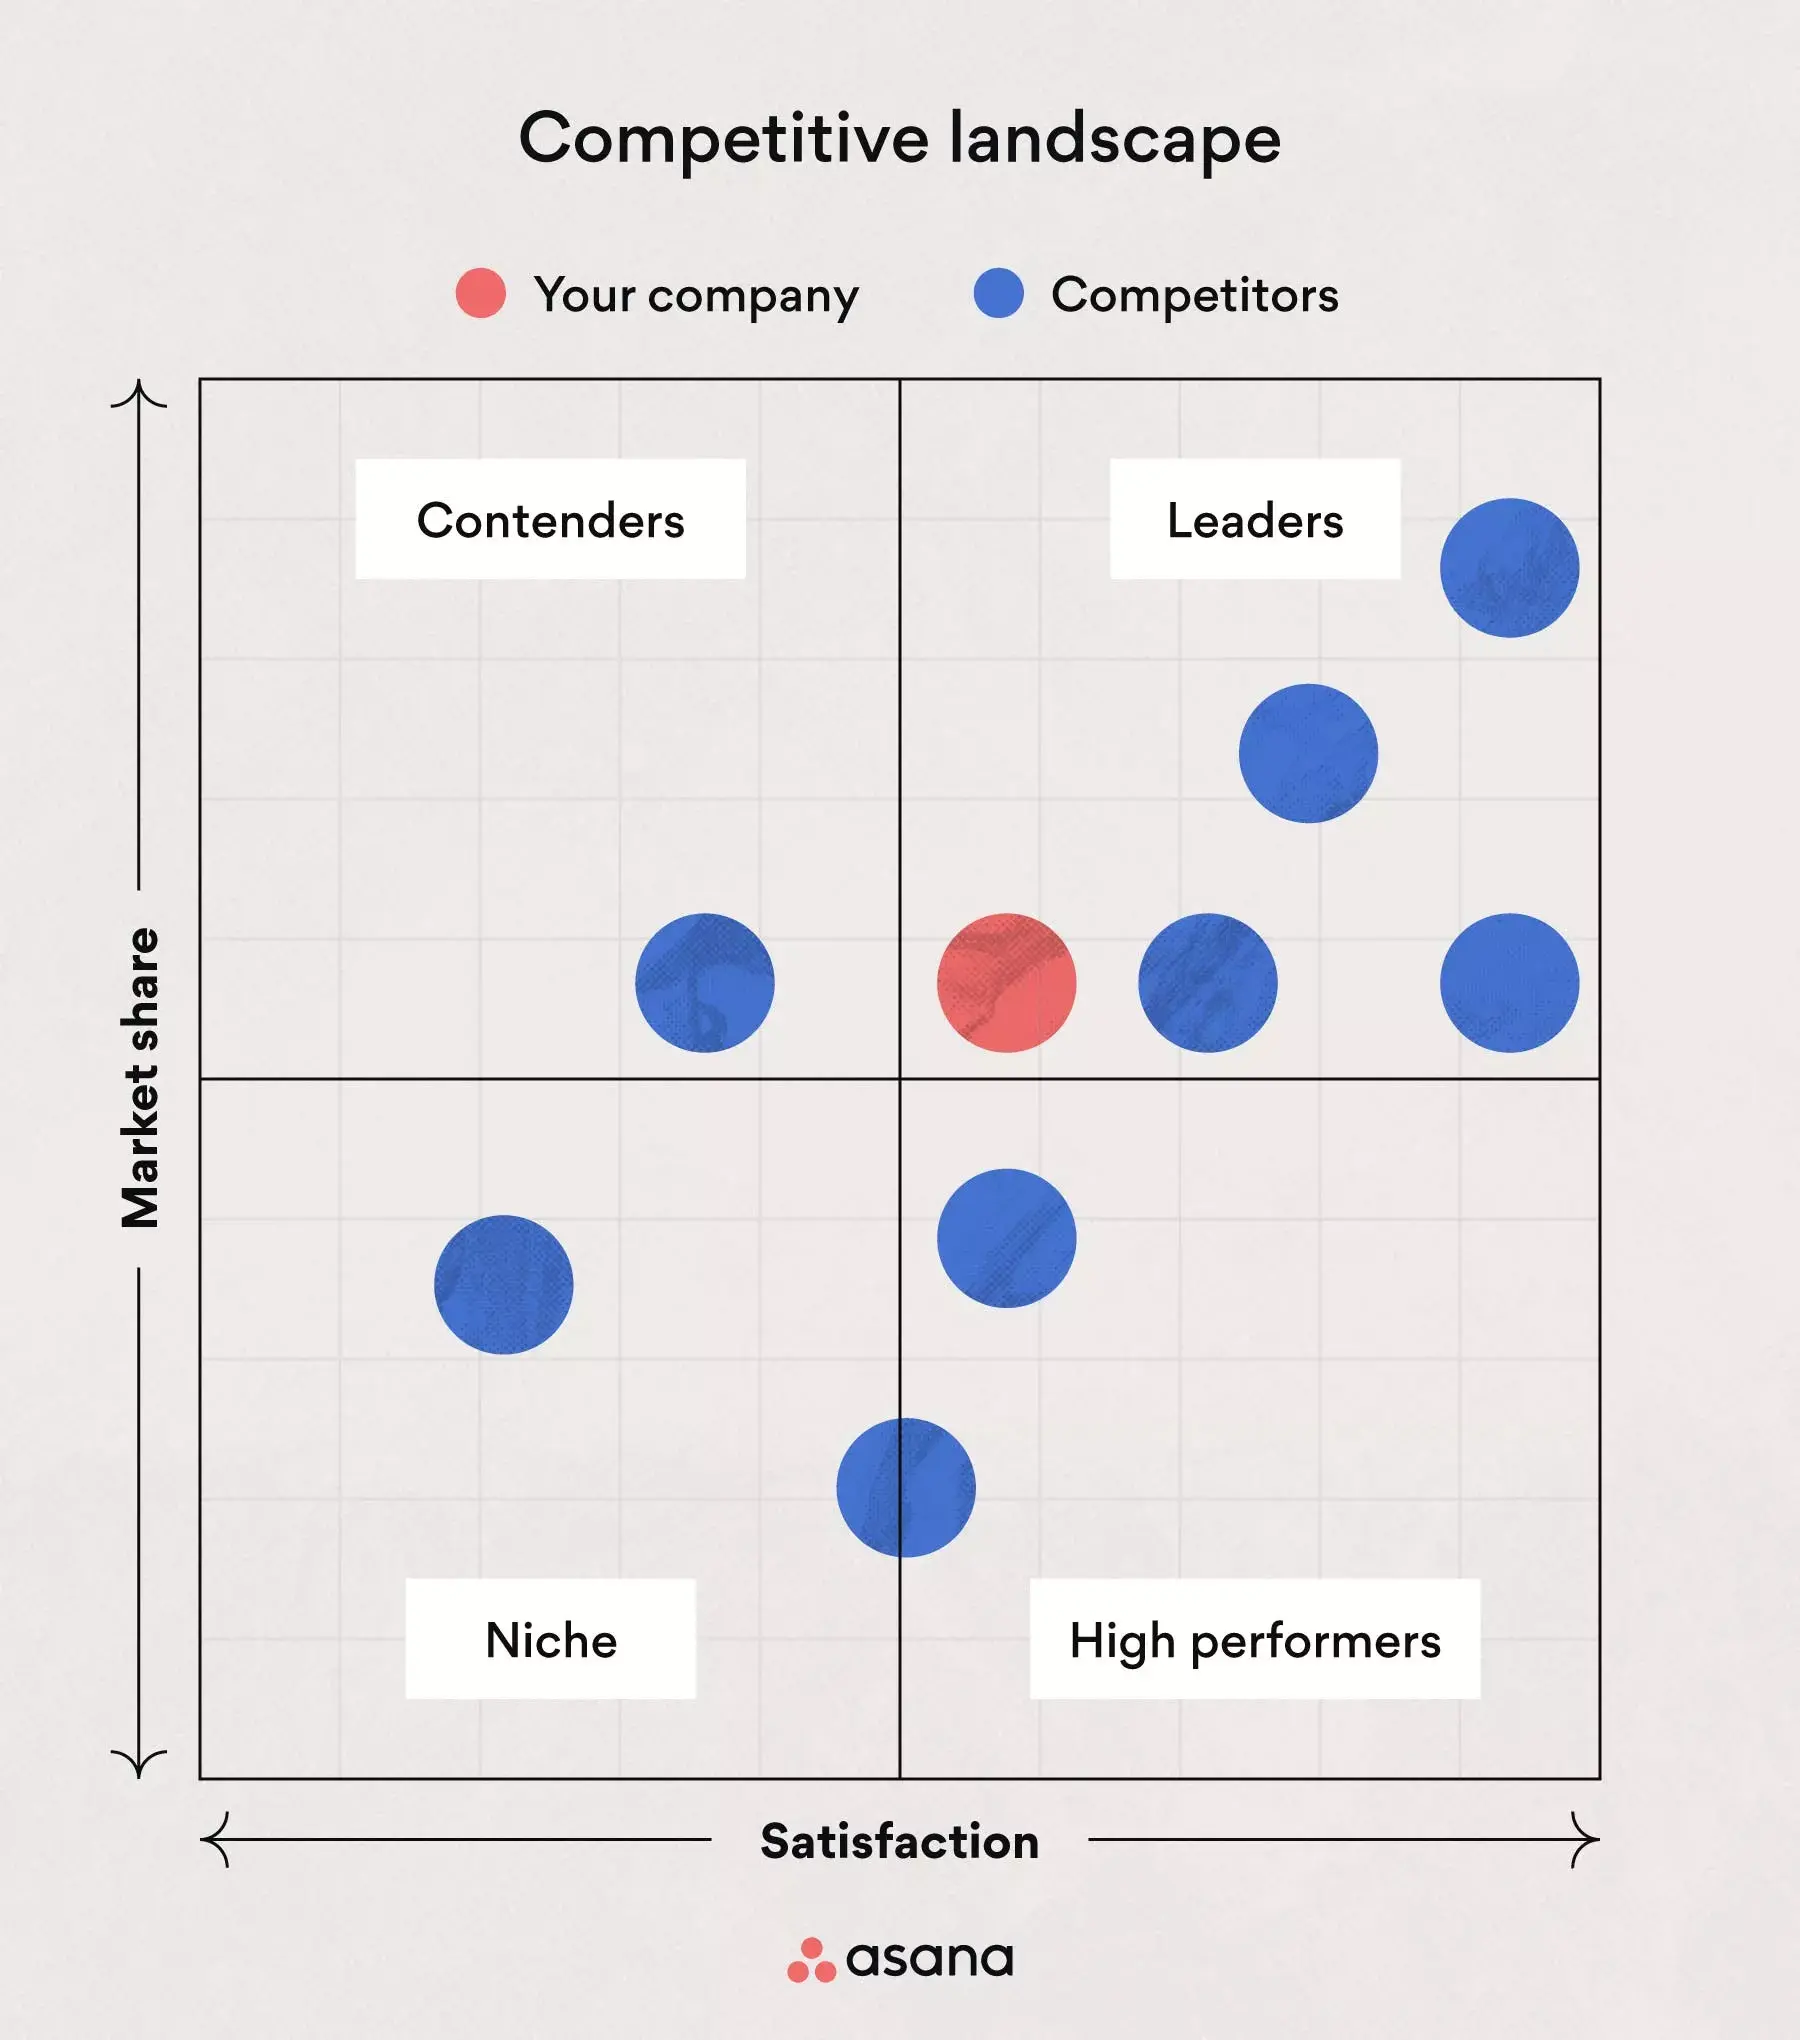
\includegraphics[width=0.5\textwidth]{examples/asana-competitive-landscape.jpg}
    \caption{Competitive Landscape by Asana}
\end{figure}

Refer to an article "How to create a competitive analysis (with
examples)" by Asana. You can use the Competitor Landscape (left image) or
Competitor Analysis Framework (right image) for your project.

\section{Literature Review}
\label{section:literature-review}

Add a literature review section if it fits with your project.